\documentclass[a4paper,showframe,11pt]{report}\usepackage[]{graphicx}\usepackage[]{color}
%% maxwidth is the original width if it is less than linewidth
%% otherwise use linewidth (to make sure the graphics do not exceed the margin)
\makeatletter
\def\maxwidth{ %
  \ifdim\Gin@nat@width>\linewidth
    \linewidth
  \else
    \Gin@nat@width
  \fi
}
\makeatother

\definecolor{fgcolor}{rgb}{0.196, 0.196, 0.196}
\newcommand{\hlnum}[1]{\textcolor[rgb]{0.063,0.58,0.627}{#1}}%
\newcommand{\hlstr}[1]{\textcolor[rgb]{0.063,0.58,0.627}{#1}}%
\newcommand{\hlcom}[1]{\textcolor[rgb]{0.588,0.588,0.588}{#1}}%
\newcommand{\hlopt}[1]{\textcolor[rgb]{0.196,0.196,0.196}{#1}}%
\newcommand{\hlstd}[1]{\textcolor[rgb]{0.196,0.196,0.196}{#1}}%
\newcommand{\hlkwa}[1]{\textcolor[rgb]{0.231,0.416,0.784}{#1}}%
\newcommand{\hlkwb}[1]{\textcolor[rgb]{0.627,0,0.314}{#1}}%
\newcommand{\hlkwc}[1]{\textcolor[rgb]{0,0.631,0.314}{#1}}%
\newcommand{\hlkwd}[1]{\textcolor[rgb]{0.78,0.227,0.412}{#1}}%
\let\hlipl\hlkwb

\usepackage{framed}
\makeatletter
\newenvironment{kframe}{%
 \def\at@end@of@kframe{}%
 \ifinner\ifhmode%
  \def\at@end@of@kframe{\end{minipage}}%
  \begin{minipage}{\columnwidth}%
 \fi\fi%
 \def\FrameCommand##1{\hskip\@totalleftmargin \hskip-\fboxsep
 \colorbox{shadecolor}{##1}\hskip-\fboxsep
     % There is no \\@totalrightmargin, so:
     \hskip-\linewidth \hskip-\@totalleftmargin \hskip\columnwidth}%
 \MakeFramed {\advance\hsize-\width
   \@totalleftmargin\z@ \linewidth\hsize
   \@setminipage}}%
 {\par\unskip\endMakeFramed%
 \at@end@of@kframe}
\makeatother

\definecolor{shadecolor}{rgb}{.97, .97, .97}
\definecolor{messagecolor}{rgb}{0, 0, 0}
\definecolor{warningcolor}{rgb}{1, 0, 1}
\definecolor{errorcolor}{rgb}{1, 0, 0}
\newenvironment{knitrout}{}{} % an empty environment to be redefined in TeX

\usepackage{alltt}
\usepackage{standalone}
\standalonetrue
\ifstandalone
  \usepackage{../../haziq_thesis}
  \usepackage{../../haziq_maths}
  \usepackage{../../haziq_glossary}
  \addbibresource{../../bib/haziq.bib}
  \externaldocument{../01/.texpadtmp/introduction}
\fi







\IfFileExists{upquote.sty}{\usepackage{upquote}}{}
\begin{document}

Data containing the number of breakdows of bovine tubercolosis (BTB) in Cornwall, the locations of the infected animals, and the year of occurence is analysed.
The interest, as motivated by veterinary epidimiology, is to understand whether or not there is spatial segregation between the herds, and whether there is a time-element to presence or absence of this spatial segregation.
There have been previous work done to analyse this data set: \hltodo{cite Diggle et al. (2005)} developed a non-parametric method to estimate spatial segregation using a multivariate point process.
The occurrences are modelled as Poisson point processes, and spatial segregation is said to have occured if the model-estimated type-specific breakdown probabilities at any given location are not significantly different from the sample proportions \hltodo{I think this is what they did - recheck}.
The authors estimated the probabilities via kernel regression, and the resulting test statistic had to be estimated via Monte Carlo methods.
Other work includes Taylor et al. (2015), who used a fully Bayes scheme for spatio-temporal multivariate log-Gaussian Cox processes.

\begin{knitrout}
\definecolor{shadecolor}{rgb}{1, 1, 1}\color{fgcolor}\begin{figure}[h]

{\centering 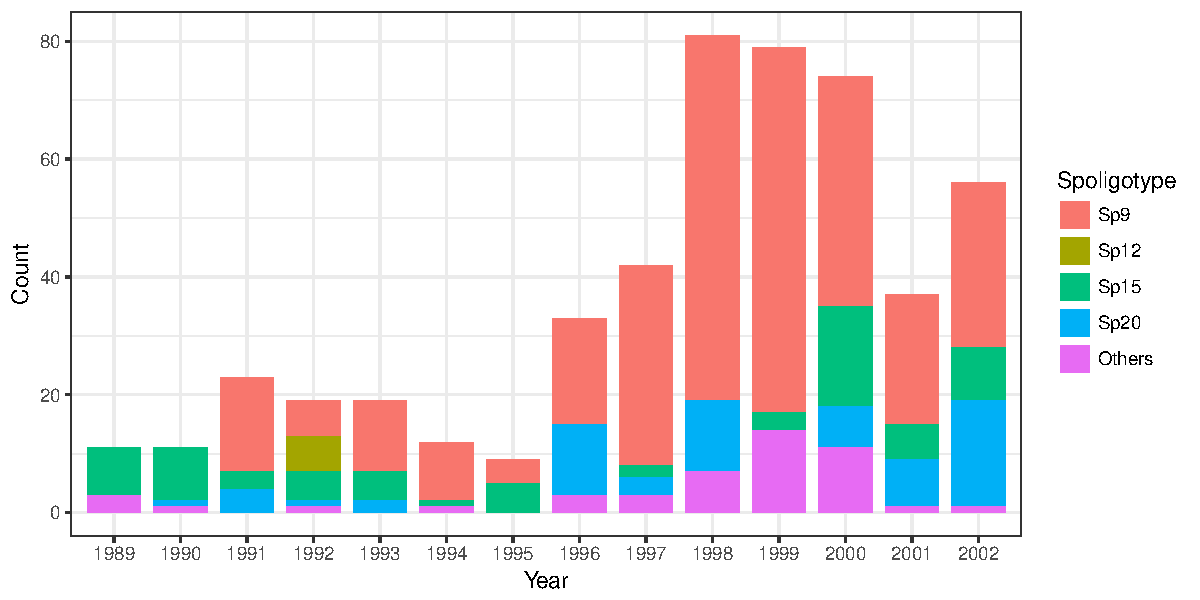
\includegraphics[width=\linewidth]{figure/plot_cow-1} 

}

\caption[Distribution of the different types (Spoligotypes) of bovine tubercolosis affecting herds in Cornwall over the period 1989 to 2002]{Distribution of the different types (Spoligotypes) of bovine tubercolosis affecting herds in Cornwall over the period 1989 to 2002.}\label{fig:plot.cow}
\end{figure}


\end{knitrout}

\hltodo{Explain data set}. $n=919$ cases in total. Originally there are 11 spoligotypes, but of these, four are most common. Therefore, the rest are combined into a separate class of `Others`. Total 14 years of data, so total number of classes is $m = 5$.

\begin{knitrout}
\definecolor{shadecolor}{rgb}{1, 1, 1}\color{fgcolor}\begin{figure}[h]

{\centering 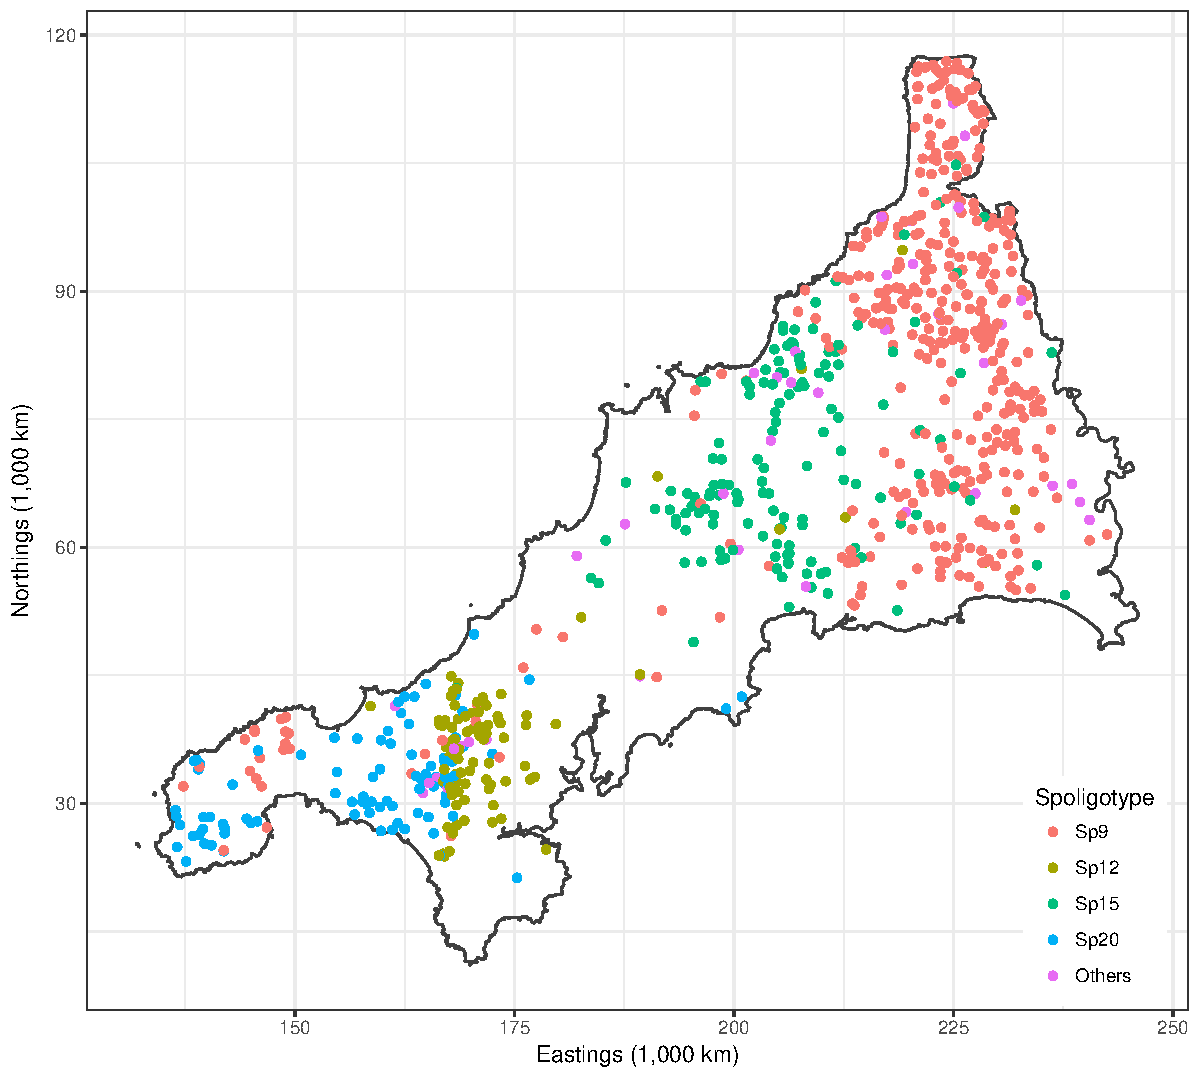
\includegraphics[width=\linewidth]{figure/plot_cornwall-1} 

}

\caption[Spatial distribution of all cases over the 14 years]{Spatial distribution of all cases over the 14 years.}\label{fig:plot.cornwall}
\end{figure}


\end{knitrout}

We are able to investigate any spatio-temporal patterns of infection using I-priors rather simply.
Let $p_{ij}$ denote the probability that a particular animal $i$ is infected with the disease with spoligotype $j \in \{1,\dots,m\}$.
We model the transformed probabilities $g(p_{ij})$ (as described in the categorical response chapter) as following a smooth function $f$ which takes two covariates: the spatial data $x_1$ (Northings and Eastings, measured in kilometres), and the temporal data $x_2$ (year of infection):
\begin{align*}
  g(p_{ij}) &= f_j(x_1, x_2) \\
  &= f_{1j}(x_1) + f_{2j}(x_2) + f_{12j}(x_1, x_2)
\end{align*}
We assume a smooth effect of space and time on the probabilities, and an appropriate RKHS for the functions $f_1$ and $f_2$ are the fBm-0.5 RKHS. Alternatively, as per Diggle et al., divide the data into four distinct time periods: 1) 1996 and earlier; 2) 1997 to 1998; 3) 1999 to 2000; and finally 4) 2001 to 2002. In this case, $x_2$ would indicate which period the infection took place in, and thus would have a nominal effect on the probabilities. An appropriate RKHS for $f_2$ in such a case would be the Pearson RKHS. In either case, the function $f_{12}$ would be the ``interaction effect'', meaning that with such an effect present, the spatial distribution of the diseases are assumed to vary across the years.

Let $h_k$, $k \in \{1,2\}$ denote the reproducing kernel of the spatial and temporal RKHSs respectively.
Then, an I-prior on $f_j$ takes the form
\begin{align*}
  f_j(x_1, x_2) &= \lambda_{1j} \sum_{i=1}^n h_1(x_1, x_{i1}) w_{ij} +
  \lambda_{2j} \sum_{i=1}^n h_2(x_2, x_{i2}) w_{ij} \\
  &\phantom{==} + \lambda_{1j} \lambda_{2j} \sum_{i=1}^n  h_1(x_1, x_{i1})h_2(x_2, x_{i2}) w_{ij}
\end{align*}
where $\bw_j = (w_{1j}, \dots, w_{nj})^\top \sim \N(0,\bI_n)$ and each of the $\bw_j$ are also independent of each other.
The parameters $\lambda_{1j}$ and $\lambda_{2j}$ are the RKHS scale parameters for the spatial and temporal covariates respectively.
Notice that the functions are indexed by the classes $j$, such that there would be $2m$ scale parameters to estimate.
This is the more general case, in which we assume \emph{separate scale} parameters in each class.
However, we may also restrict the scale parameters to be equivalent in each class, so that this so-called \emph{shared scale} model has only two parameters to estimate, which is simpler to do inference.
Note that there are also intercept parameters to estimate (one in each class), but these will not be reported as they are irrelevant to the discussion at hand.

Spatio-temporal effects of the BTB breakdowns can be easily inferred through the RKHS scale parameters.
The hypothesis of temporal significance is the same as testing the significance of the $\lambda_2$ parameter, while the test of both spatial and temporal effects are conducted on $\lambda_1$ and $\lambda_2$ simultaneously (equivalent to modelling $f$ with a constant).
For these tests, it is simpler to infer from the shared scale model, for which we can read the results directly of off Table \ref{tab:table.btb}.
The said table displays the posterior mean estimate of the scale parameters, and together with its posterior standard deviation.
From Chapter X, we know that these scale parameters follow a normal posterior distribution, so we can calculate the $Z$-scores by dividing the mean by its corresponding s.d..
Absolute values greater than three would satisfy a Bayesian hypothesis test of significance at the 0.01 level, for which we see all parameters satisfy in the shared scale model.


\begin{landscape}\begin{table}

\caption{\label{tab:table.btb}Results of the fitted I-probit models.}
\centering
\begin{tabular}[t]{lrrrlrrrlrrrl}
\toprule
\multicolumn{ 1}{c}{\bfseries  } & \multicolumn{12}{c}{\bfseries Model} \\
\cmidrule(l{2pt}r{2pt}){2-13}
\multicolumn{1}{c}{ } & \multicolumn{3}{c}{Spatial} & \multicolumn{1}{c}{ } & \multicolumn{3}{c}{Spatio-temporal} & \multicolumn{1}{c}{ } & \multicolumn{3}{c}{Spatio-period} \\
\cmidrule(l{2pt}r{2pt}){2-4} \cmidrule(l{2pt}r{2pt}){6-8} \cmidrule(l{2pt}r{2pt}){10-12}
  & Estimate & S.D. & |$Z$|-score &  & Estimate & S.D. & |$Z$|-score &  & Estimate & S.D. & |$Z$|-score & \\
\midrule
\addlinespace[0.5em]
\multicolumn{13}{l}{\textbf{Shared scale model}}\\
\hspace{1em}Spatial & 0.19 & 0.003 & 64.9 & *** & 0.18 & 0.003 & 67.4 & *** & 0.19 & 0.003 & 65.6 & ***\\
\hspace{1em}Temporal &  &  &  &  & 0.01 & 0.000 & 16.5 & *** & 0.00 & 0.000 & 12.0 & ***\\
\addlinespace[0.5em]
\multicolumn{13}{l}{\textbf{Separate scale model}}\\
\hspace{1em}Spatial (Sp9) & 0.47 & 0.014 & 33.5 & *** & 0.48 & 0.014 & 33.1 & *** & 0.47 & 0.014 & 33.9 & ***\\
\hspace{1em}Spatial (Sp12) & 0.19 & 0.007 & 29.2 & *** & 0.26 & 0.008 & 31.4 & *** & 0.23 & 0.007 & 31.3 & ***\\
\hspace{1em}Spatial (Sp15) & 0.17 & 0.005 & 33.9 & *** & 0.17 & 0.005 & 33.6 & *** & 0.17 & 0.005 & 33.9 & ***\\
\hspace{1em}Spatial (Sp20) & 0.16 & 0.004 & 44.2 & *** & 0.17 & 0.004 & 39.6 & *** & 0.17 & 0.004 & 40.7 & ***\\
\hspace{1em}Spatial (Others) & 0.00 & 0.004 & 0.0 &  & 0.00 & 0.004 & 0.0 &  & 0.00 & 0.004 & 0.0 & \\
\hspace{1em}Temporal (Sp9) &  &  &  &  & 0.00 & 0.002 & 0.1 &  & 0.00 & 0.001 & 6.3 & ***\\
\hspace{1em}Temporal (Sp12) &  &  &  &  & 0.01 & 0.001 & 17.8 & *** & 0.01 & 0.001 & 12.4 & ***\\
\hspace{1em}Temporal (Sp15) &  &  &  &  & 0.02 & 0.001 & 12.3 & *** & 0.00 & 0.001 & 0.0 & \\
\hspace{1em}Temporal (Sp20) &  &  &  &  & 0.00 & 0.002 & 0.1 &  & 0.00 & 0.001 & 0.1 & \\
\hspace{1em}Temporal (Others) &  &  &  &  & 0.00 & 0.002 & 0.0 &  & 0.01 & 0.001 & 10.9 & ***\\
\bottomrule
\multicolumn{13}{l}{\textsuperscript{*} Lower-bound values (Brier scores) for the shared scale model are -664.8 (0.143), -654.9 (0.135), and -663.7 (0.136) respectively.}\\
\multicolumn{13}{l}{\textsuperscript{\dag} Lower-bound values (Brier scores) for the separate scale model are -660.8 (0.138), -667.9 (0.129), and -678.3 (0.130) respectively.}\\
\end{tabular}
\end{table}
\end{landscape}



A similar conclusion is reached when inferring from the separate scale model. Instead of individual tests of significance, we now need to test
\[
  \text{H}_0: \lambda_1 = \dots = \lambda_m = 0.
\]

We know that by the mean-field approximation used, the $\lambda_j$s are independent of each other, and therefore a $\chi^2$ test statistic can be built via
\[
  \chi^2 = \sum_{j=1}^m Z_j^2
\]
which is then compared against extreme values of the $\chi^2_m$-distribution.
As is often the case, separate scale models tend to fit the data better as it gives more generality due to having different scale parameters in each class.
This is also the case for the BTB data, where we see from the footnotes of Table \ref{tab:table.btb} that the Brier scores for the separate scale models are better than the Brier scores in the shared scale models.
For all following plots, we made use of the separate scale model for predicting the surface probabilities. Another comment regarding the models is that the conclusion remains the same if we had used the periodic formulation for $x_2$.

\begin{knitrout}
\definecolor{shadecolor}{rgb}{1, 1, 1}\color{fgcolor}\begin{figure}[h]

{\centering 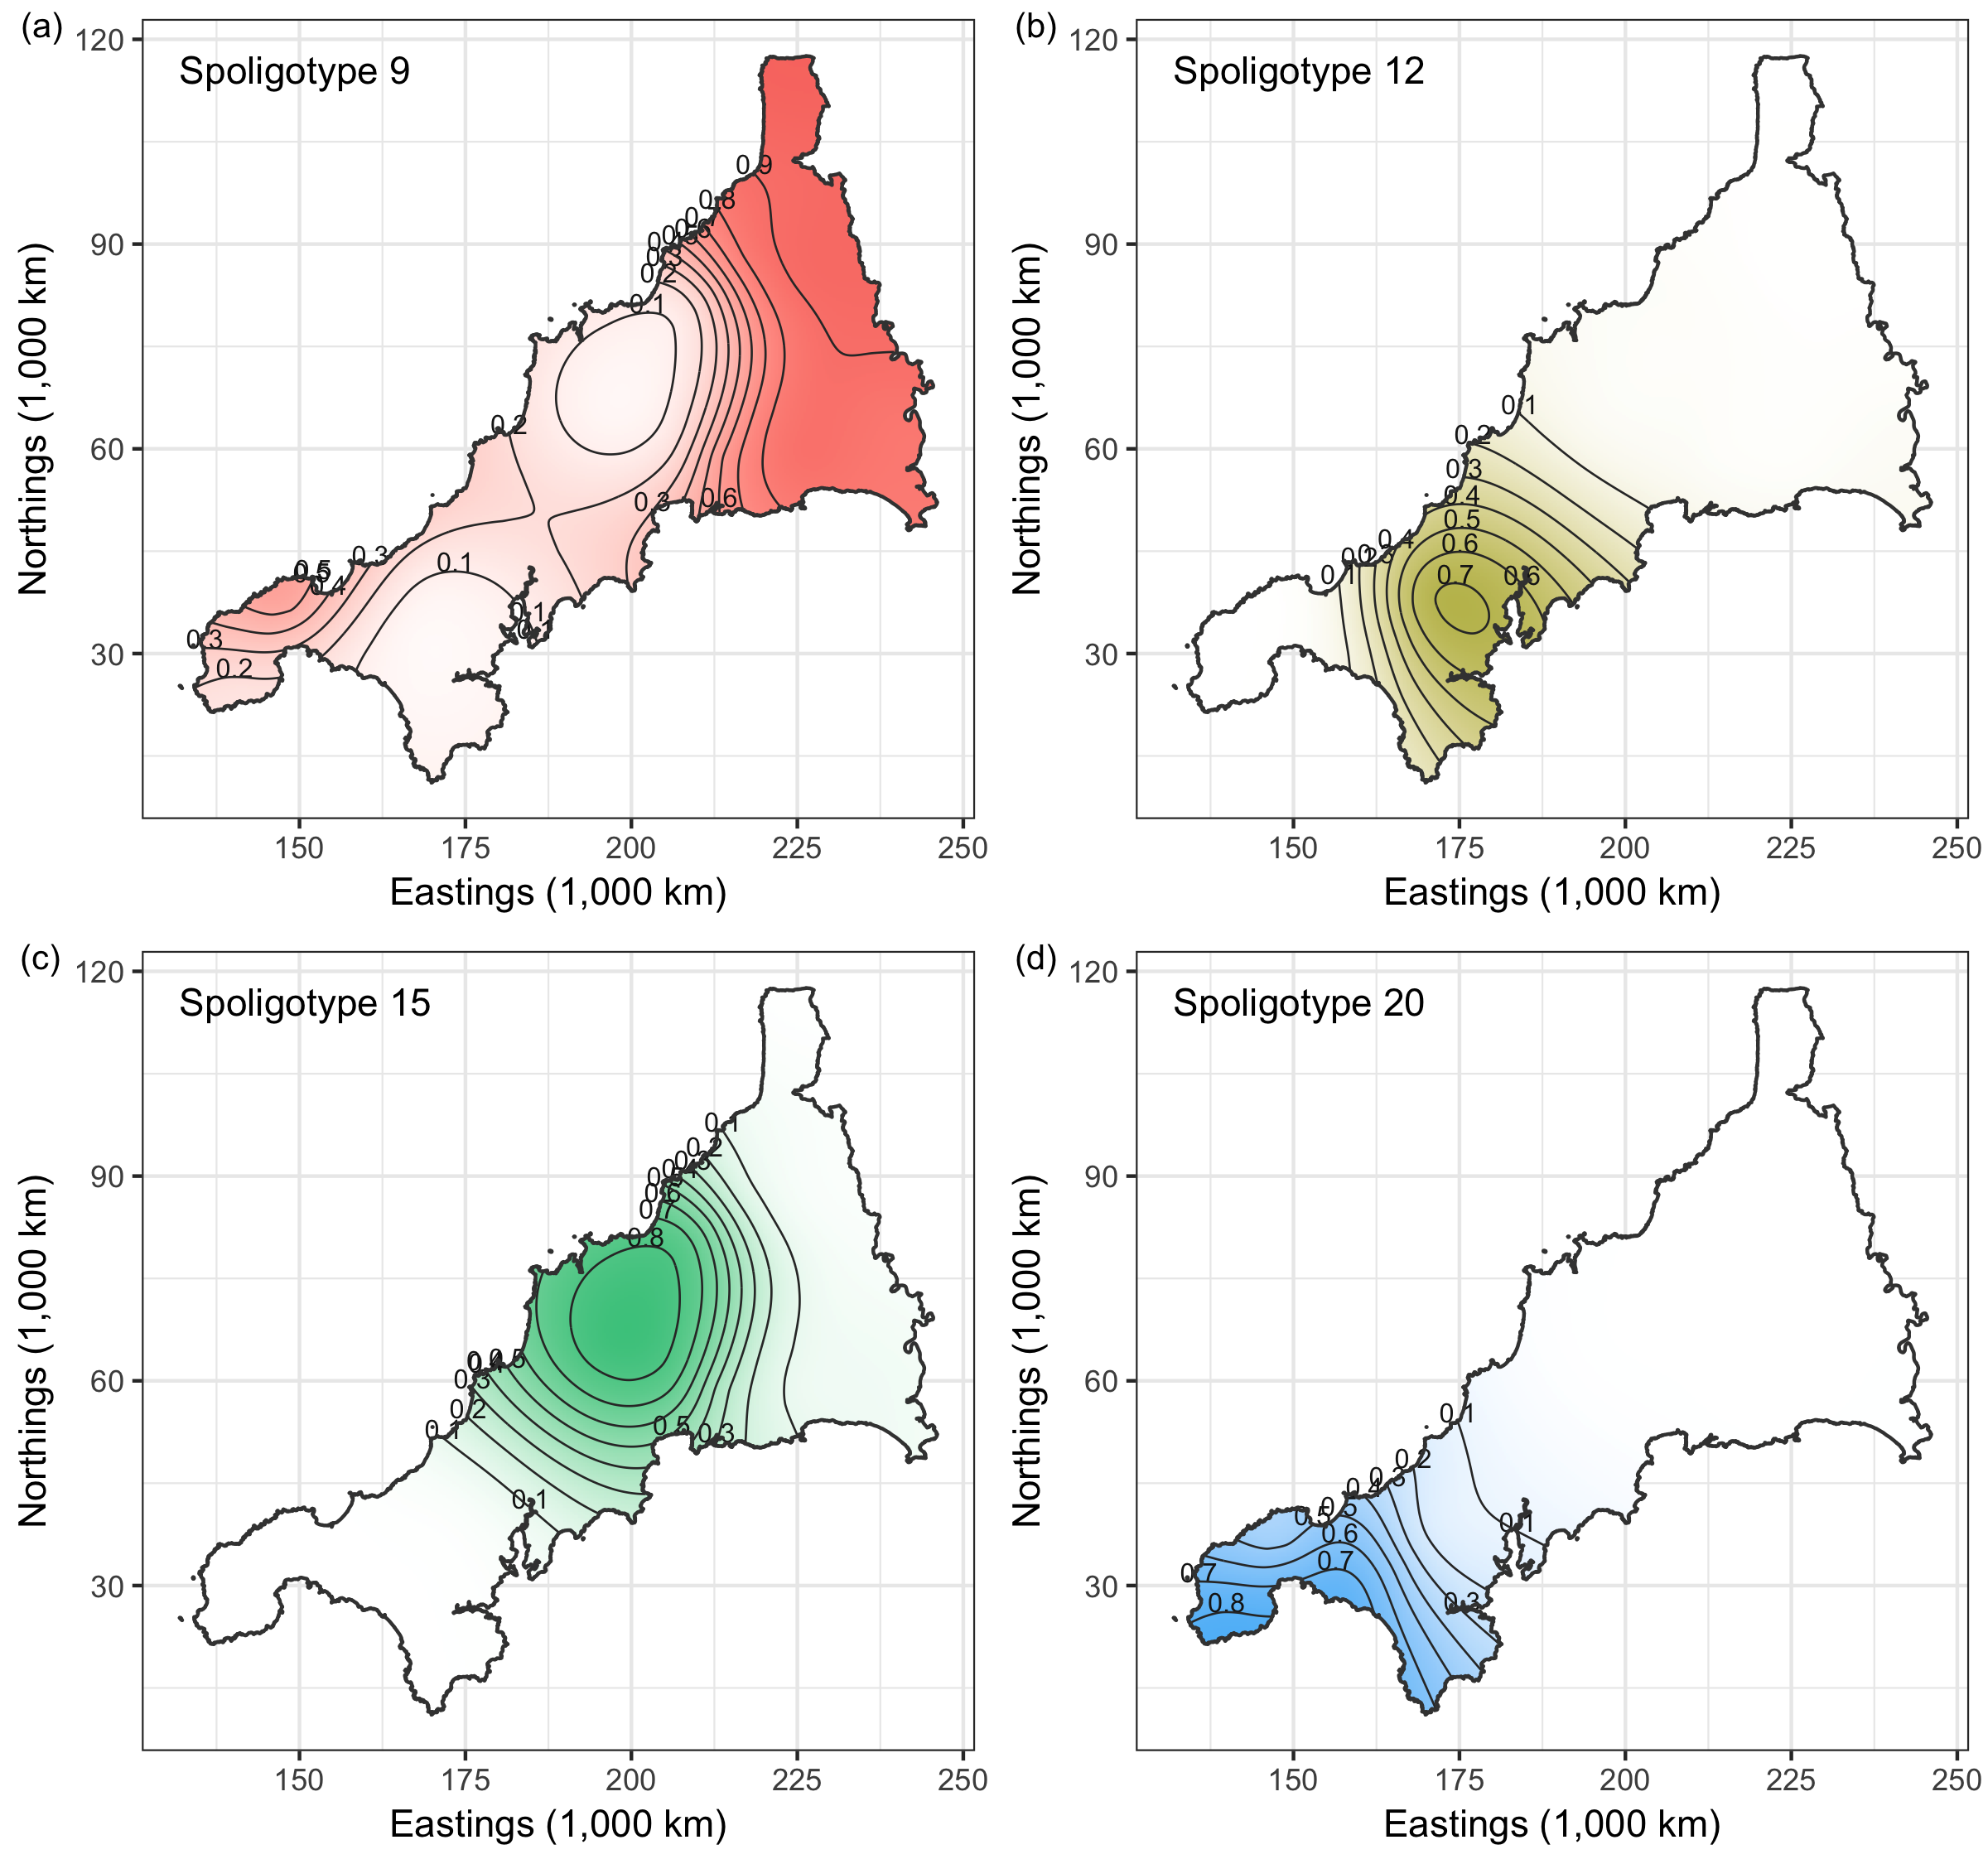
\includegraphics[width=\linewidth]{figure/plot_btb-1} 

}

\caption[Caption]{Caption.}\label{fig:plot.btb}
\end{figure}


\end{knitrout}

For a more visual approach, we can look at the plots of the surface probabilities.
To obtain these probabilities, we first determined the spatial points (Northings and Eastings) which fall inside the polygon which makes up Cornwall.
We then obtained predicted probabilities for each class of disease at each location.
Figure \ref{fig:plot.btb} was obtained using the model with spatial covariates only, thus ignoring any temporal effects.
In the case of the spatio-temporal model, we used the model which had the period formulation for time.
This way, we can obtain the surface probabilities in only four time periods, although there is no issue with using the continuous time model.
It is more economical to display four plots rather than the 14 yearly plots within the margins of this thesis.

As the model suggests, there is indeed spatial segregation for the four most common spoligotypes, and this is also very prominently seen from Figure \ref{fig:plot.btb}.
In comparing the distribution of the spoligotypes over the years, we may refer to Figure \ref{fig:plot.temporal.btb}.
For each time period, we superimpose the actual observations onto the predicted surface probabilities.
In addition, coloured dotted lines are displayed to indicate the ``decision boundaries'' for each of the four spoligotypes.
The most evident change is seen to the spatial distribution of spoligotype 12, with the decision boundary giving it a large area in years 1996 and earlier, but this steadily shrunk over the years.
Spoligotype 9, which is most commonly seen in the east of Cornwall, seems to have made its way down to the south-west over the years.
The other two spoligotypes seem to be rather constant over the years.
This is supported also by the spatio-period model results in Table \ref{tab:table.btb}, where the test of nullity for the scale parameters of these two spoligotypes are not rejected.

\begin{knitrout}
\definecolor{shadecolor}{rgb}{1, 1, 1}\color{fgcolor}\begin{figure}[h]

{\centering 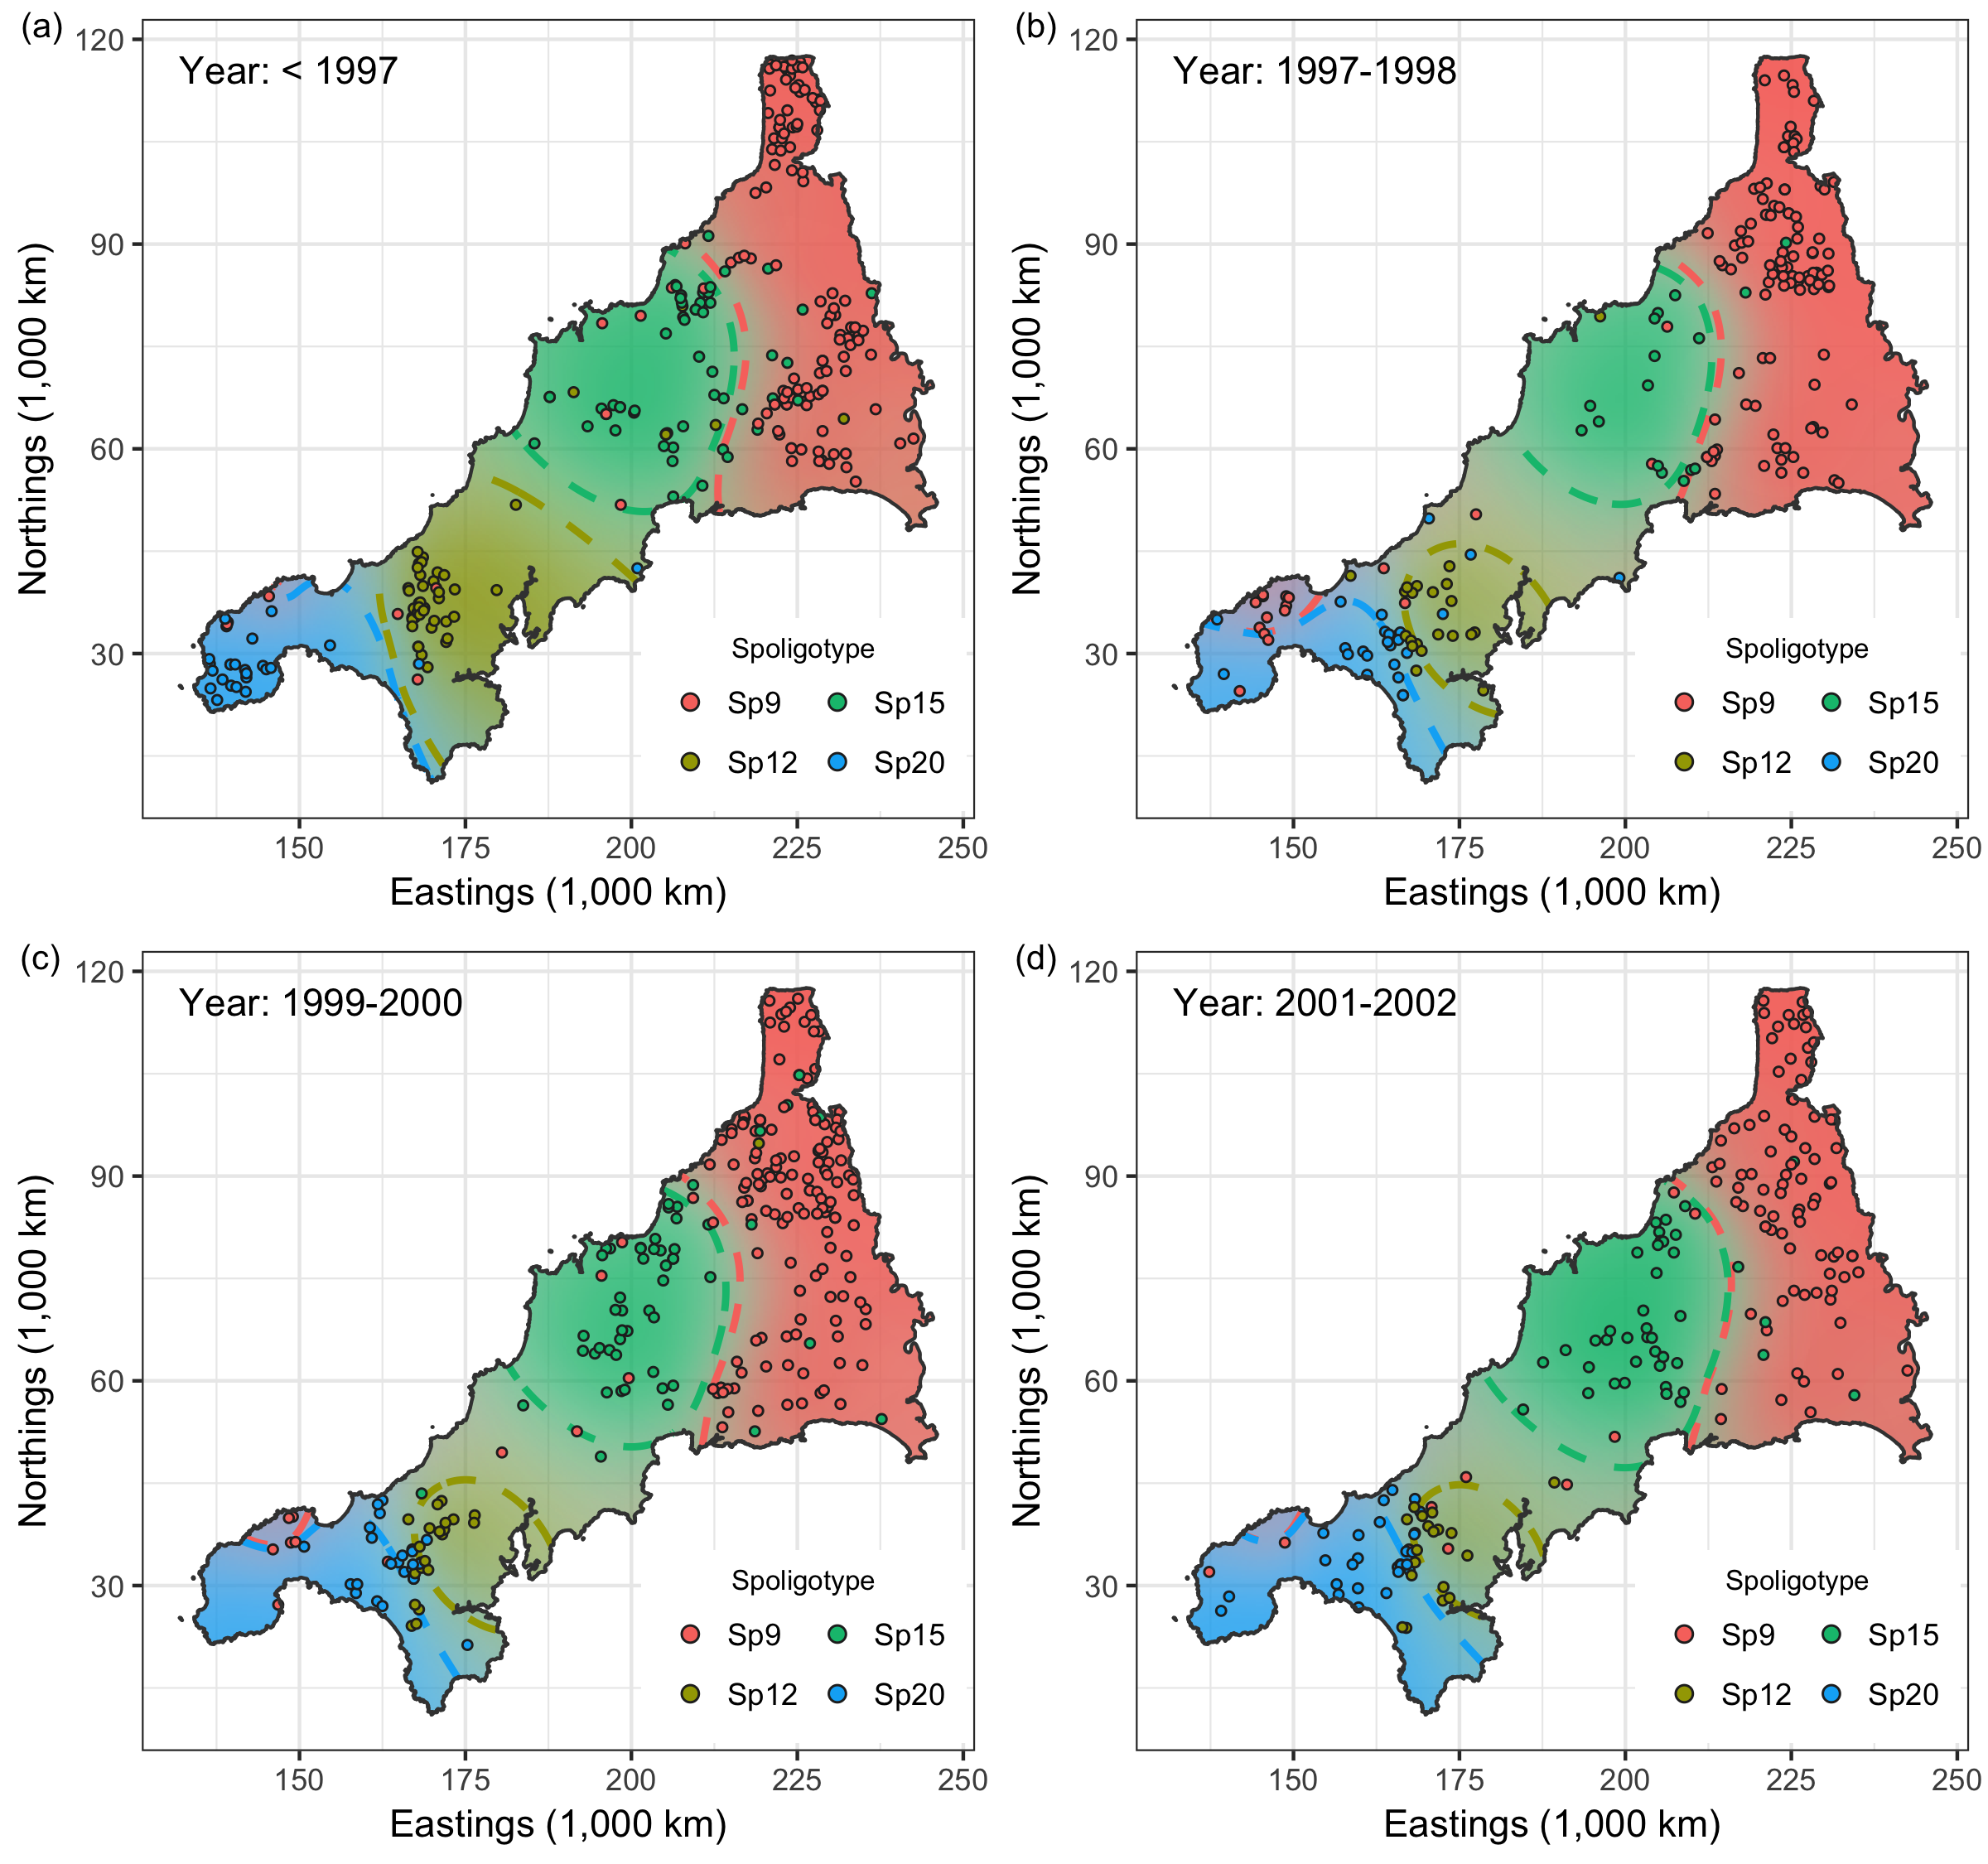
\includegraphics[width=\linewidth]{figure/plot_temporal_btb-1} 

}

\caption[Caption]{Caption.}\label{fig:plot.temporal.btb}
\end{figure}


\end{knitrout}

\end{document}


